%# -*- coding: utf-8-unix -*-
%%==================================================
\chapter{多任务联合学习}

\section{Multi-Task Learning Using Uncertainty to Weigh Losses for Scene Geometry and Semantics}

论文地址: \href{https://arxiv.org/abs/1705.07115v3}{Multi-Task Learning Using Uncertainty to Weigh Losses for Scene Geometry and Semantics}

参考资料: \href{https://zhuanlan.zhihu.com/p/65137250}{多任务损失优化1},\href{https://blog.csdn.net/cdknight_happy/article/details/102618883}{多任务损失优化2},\href{https://blog.csdn.net/qq_41214679/article/details/110750812}{多任务损失优化3}

\subsection{问题提出}

\subsubsection{多任务学习介绍}

以前多任务的总损失函数可用如下表达式表示
\begin{align}
& L_{total} = \sum_i w_iL_i
\end{align}

只是简单的对每个子任务进行线性求和,这样会存在很多问题,例如模型对于权重参数很敏感,如下图\href{fig:1-1}{1-1}所示
\begin{figure}
  \centering
  % Requires \usepackage{graphicx}
  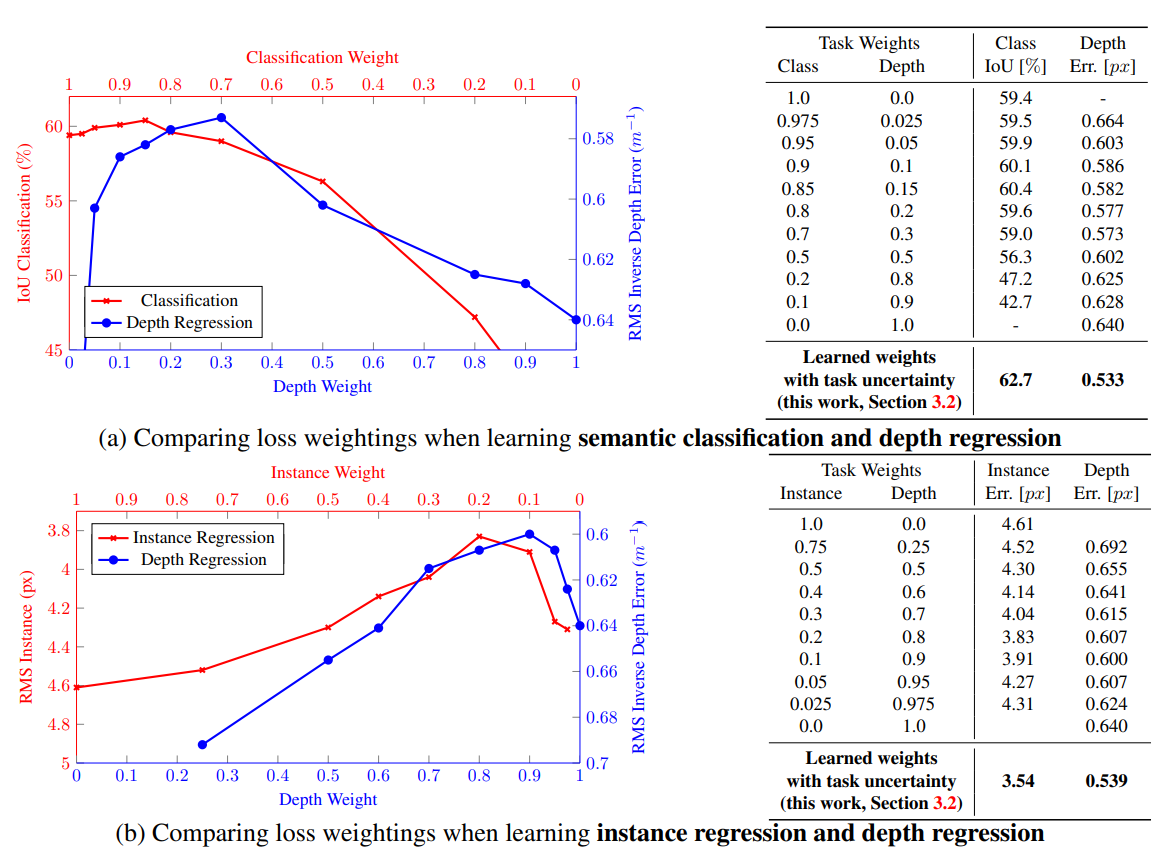
\includegraphics[width=4.5in]{figure/example/2.png}\\
  \caption{不同任务对权重参数很敏感}
  \label{fig:1-1}
\end{figure}

\subsubsection{本文创新点}

多任务联合学习可以提升各任务的学习效果,因为多任务可以共享数据集、共享低层特征。但多任务联合学习时,该如何对各子任务的损失函数进行加权才能取得最优的训练效果,这是本文所关心的问题。

本文中作者提出的多任务如下图\href{fig:1-2}{1-2}所示:
\begin{figure}
  \centering
  % Requires \usepackage{graphicx}
  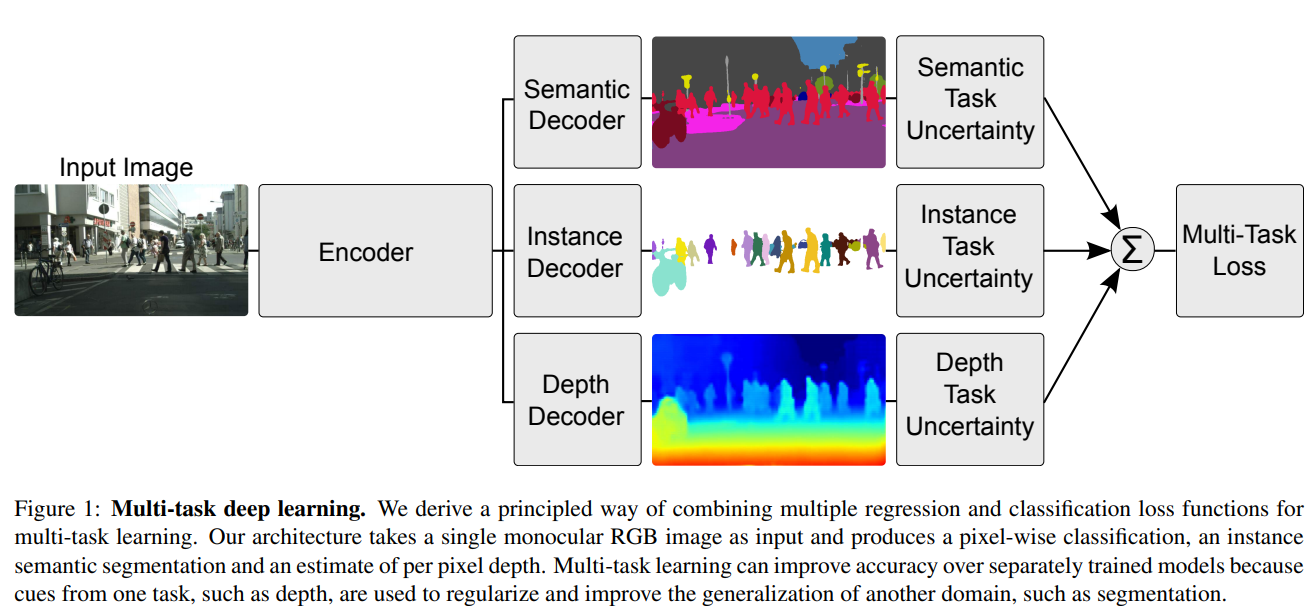
\includegraphics[width=5.5in]{figure/example/1.png}\\
  \caption{论文中用到的多任务图}
  \label{fig:1-2}
\end{figure}

本论文创新点:
\begin{enumerate}
    \item 利用同方差不确定性同时学习不同数量和单元的分类和回归损失的一种新颖多任务损失
    \item 建立统一的组合语义分割、定位分割和深度回归体系结构
    \item 证明模型损失权重的重要性,并且能够解决并获得良好的参数。
\end{enumerate}

\subsection{解决方案}

\subsubsection{多任务似然}
下面通过最大化同方差不确定性的最大高斯似然估计来推导多任务损失函数。

假设输入数据为X,参数矩阵为W,模型输出为$f^W(x)$,真实输出为$y$,这里的$f^W(x)$可以理解成多个子任务的输出汇总。

1、对于回归任务,定义其概率是以输出为均值的高斯似然,即
\begin{align}
& p(y|f^W(x)) = N(f^W(x),\sigma^2)
\end{align}
这个函数可以理解成:真实输出$y$和输出值$f^W(x)$之间(也就是误差)服从正态分布,标准差为$\sigma$

2、对于分类任务,通过Softmax将输出转化为概率,即:
\begin{align}
& p(y|f^W(x)) = Softmax(f^W(x))
\end{align}

3、对于多任务模型(输出是相互独立的),其似然为:
\begin{align}
& p(y_1,...,y_k|f^W(x)) = p(y_1|f^W(x))...p(y_K|f^W(x))
\end{align}

其中

正态分布的概率密度函数为
\begin{align}
& f(x) = \frac{1}{\sqrt{2 \pi}\sigma}exp(-\frac{(x - \mu)^2}{2\sigma^2})
\end{align}

Softmax表达式为
\begin{align}
& softmax(X)_{ij} = \frac{exp(X_{ij})}{\sum_k exp(X_{ik})}
\end{align}

\subsubsection{回归任务}

对于回归任务,即公式(2),其对数似然为:
\begin{align}
&\log p(y|f^W(x)) \propto - \frac{1}{2\sigma^2}||y - f^W(x)||^2 - log \sigma
\end{align}

其中,$\sigma$是高斯似然的标准差,也是模型的噪声参数,表示输出数据中的噪声量。我们的目的是基于参数矩阵$W$和标准差$\sigma$最大化对数似然。

假设多任务模型进行两个回归任务,两个任务都符合高斯分布,输出分别是 $y_1$和$y_2$,那么总的对数似然为:
\begin{align}
&p(y_1,y_2 | f^W(x)) = p(y_1|f^W(x))p(y_2|f^W(x)) \nonumber \\
&= N(y_1;f^W(x),\sigma^2_1)N(y_2;f^W(x),\sigma^2_2)
\end{align}

取对数,优化目标变成了最大化对数似然,也是最小化负对数似然,即:
\begin{align}
& = -\log p(y_1,y_2 | f^W(x)) \nonumber \\
&\propto \frac{1}{2\sigma^2_1}||y_1 - f^W(x)||^2 + \frac{1}{2\sigma^2_2}||y_2 - f^W(x)||^2 + \log \sigma_1 \sigma_2 \nonumber \\
& = \frac{1}{2\sigma^2_1}L_1(w) + \frac{1}{2\sigma^2_2}L_2(w) + \log \sigma_1 \sigma_2
\end{align}

要是想最小化负对数似然,就需要调整$\sigma_1$ 和 $\sigma_2$的值。 $\sigma_1$ 增加,$L_1(w)$会减小,反之亦然。最后项影响不大,可以当作正则化项。

\subsubsection{分类任务}

对于分类任务的概率,添加一个标量缩放系数$\sigma^2$
\begin{align}
&p(y|f^W(x),\sigma) = Softmax(\frac{1}{\sigma^2}f^W(x))
\end{align}

这被称作是Boltzmann分布,也叫做吉布斯分布。系数$\sigma^2$可以是设定的,也可以是通过学习得到的,决定离散分布的平坦程度。该值和分布的不确定性(熵)有关。其对数似然可以写成:
\begin{align}
log(y=c|f^W(x),\sigma) = \frac{1}{\sigma^2}f_c^W(x) - log(\sum_{c'}exp(\frac{1}{\sigma^2}f^W_{c'}(x)))
\end{align}

\subsubsection{回归和分类任务}
假设一个多任务模型由一个分类任务和一个回归任务组成,那么联合损失为:
\begin{align}
& -\log p(y_1,y_2 = c|f^W(x)) \nonumber \\
& = - \log N(y_1;f^W(x),\sigma_1^2) \cdot Softmax(y_2 = c;f^W(x),\sigma_2) \nonumber \\
& = \frac{1}{2\sigma^2_1}||y_1 - f^W(x)||^2 + log\sigma_1 - \log p(y_2 = c | f^W(x),\sigma_2) \nonumber \\
& = \frac{1}{2\sigma^2_1}L_1(W) +\frac{1}{\sigma^2_2}L_2(W)+ \log \sigma_1+ \log\frac{\sum_{c'}exp(\frac{1}{\sigma^2_2}f_{c'}^W(x))}{(\sum_{c'}exp(f_{c'}^W(x))^{\frac{1}{\sigma^2_2}}}\nonumber \\
&\approx \frac{1}{2\sigma_1^2}L_1(W) + \frac{1}{\sigma^2_2}L_2(W)+\log\sigma_1+ \log\sigma_2
\end{align}

上式中,$L_1(W) = || y_1-f^W(x)||^2$,为回归子任务输出和真实label = $y_1$ 间的欧式距离。 $L_2(W)=-\log (Softmax( y_2 , f^W(x)))$是分类子任务的交叉熵损失。对于最后一项,我们假设是约等的,即
\begin{align}
& \frac{1}{\sigma_2}\sum_{c'}exp(\frac{1}{\sigma^2_2}f_{c'}^W(x)) \approx (\sum_{c'}exp(f_{c'}^W(x))^{\frac{1}{\sigma^2_2}}
\end{align}

当$\sigma_2 = 1$时,上式等号成立。优化的目的是同时寻找最优的$W$、$\sigma_1$和$\sigma_2$。

最终的目标可以看成是学习每一个子任务输出的相对权重。大的$\sigma_2$会降低$L_2(W)$的影响,小的$\sigma_2$会增大$L_2(W)$的影响。

作者最终的做法是在模型训练的过程中去优化$\sigma_1$和$\sigma_2$,并且为了提升数值稳定性,作者去学习参数$s:=\log \sigma^2$。


\subsection{实验结果}

实验结果如图\href{fig:1-3}{1-3}所示, 得出的结论是基于三个任务的不确定性进行损失加权的效果最好。
\begin{figure}
  \centering
  % Requires \usepackage{graphicx}
  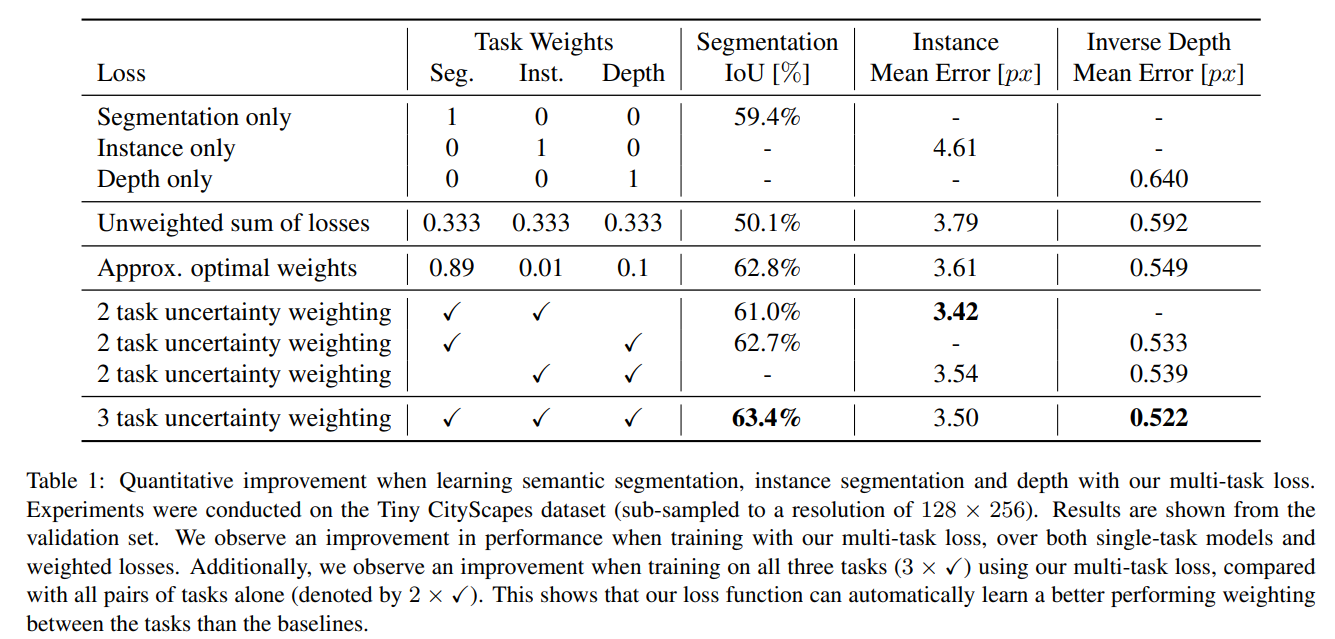
\includegraphics[width=5in]{figure/example/3.png}\\
  \caption{实验结果图}
  \label{fig:1-3}
\end{figure}

\subsection{参考代码}

多任务联合学习的特点是不同子任务共享低层特征,并通过不同子任务的协同学习进行信息的交互,在相互促进中完成整个任务。举个计算机视觉的例子,在计算机视觉感知上,任务级别从低到高可以划分为:物体分类,目标检测,语义分割和实例分割。如果想通过端到端方式训练整个模型,完成所有任务,我们必须为这些任务分配合理的权重。假设目标检测和语义分割可以实现端到端学习的话,那么如果目标检测在训练上表现的效果很差,语义分割的效果也不会好到哪去。我们在训练模型完成多个任务时,期待这些相互协同的任务是往相互促进的方向发展,而不是相互制约。

在作者给出的参考代码中,以两个回归任务联合学习为例,其对应的联合损失如下:

\begin{align}
& = -\log p(y_1,y_2 | f^W(x)) \nonumber \\
&\propto \frac{1}{2\sigma^2_1}||y_1 - f^W(x)||^2 + \frac{1}{2\sigma^2_2}||y_2 - f^W(x)||^2 + \log \sigma_1 \sigma_2 \nonumber \\
& = \frac{1}{2\sigma^2_1}L_1(w) + \frac{1}{2\sigma^2_2}L_2(w) + \log \sigma_1 \sigma_2
\end{align}

假设我们手头上有服从正态分布的,样本数为1024一维随机样本$X$,通过这些样本,我们分别添加了方差为10,方差为1的线性随机噪声$y1$,$y2$,如图\href{fig:1-4}{1-4}所示。
\begin{figure}
  \centering
  % Requires \usepackage{graphicx}
  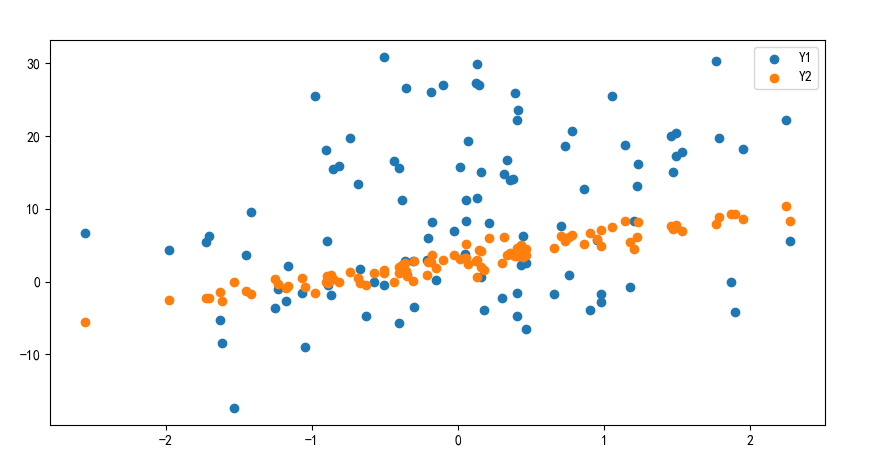
\includegraphics[width=5in]{figure/example/4.png}\\
  \caption{方差为10,方差为1的线性随机噪声y1,y2}
  \label{fig:1-4}
\end{figure}

\begin{lstlisting}[language={C}, caption={数据生成代码}]
 '''Evaluate on synthetic data'''
N = 100
nb_epoch = 2000
batch_size = 20
nb_features = 1024
Q = 1
D1 = 1  # first output
D2 = 1  # second output

def gen_data(N):
    X = np.random.randn(N, Q)
    w1 = 2.
    b1 = 8.
    sigma1 = 1e1  # ground truth 方差为10
    Y1 = X.dot(w1) + b1 + sigma1 * np.random.randn(N, D1)  #添加方差为10的线性随机噪声
    w2 = 3.
    b2 = 3.
    sigma2 = 1e0  # ground truth 方差为1
    Y2 = X.dot(w2) + b2 + sigma2 * np.random.randn(N, D2)  #添加方差为1的线性随机噪声
    return X, Y1, Y2
\end{lstlisting}

接着我们定义一个简单的模型来同时拟合这两组数据。因为输入的样本维数只有1维,因此我们定义一个神经元作为输入层,接着定义一个含1024个神经元的全连接层,并在每个单元后连接一个Relu非线性激活函数,进行特征提取。整个全连接层可以对一个样本提取1024维的特征。

接着我们定义两个神经元作为输出层,这两个神经元分别代表两个子任务,这两个子任务共享前面隐藏层提取的特征,并分别对方差为10,方差为1的线性随机噪声进行拟合。

接下来就是本文的重点了:我们根据式子\href{1-14}{1-14},定义一个MultiLoss层,并将输出层中两个神经元作为输入,核心代码如下所示。

\begin{lstlisting}[language={C}, caption={MultiLoss Layer核心代码}]
 def multi_loss(self, ys_true, ys_pred):
        assert len(ys_true) == self.nb_outputs and len(ys_pred) == self.nb_outputs
        loss = 0
        #这里以两个回归任务为例
        for y_true, y_pred, log_var in zip(ys_true, ys_pred, self.log_vars):
            precision = (K.exp(-log_var[0]))
            loss += K.sum(precision * (y_true - y_pred) ** 2. + log_var[0], -1)

        return K.mean(loss)
\end{lstlisting}

最后输出结果为$[\frac{1}{\sigma_1^2} = 8.648183872325495, \frac{1}{\sigma_2^2} = 0.9251061404392964]$,分别对应在方差为10,方差为1线性随机噪声下损失函数的权值。我们可以发现,线性随机噪声的方差越大,信息的不确定性越大,子任务的损失函数被赋予的权值也就越大。整个模型如图\href{fig:1-5}{1-5} 所示。

\begin{figure}
  \centering
  % Requires \usepackage{graphicx}
  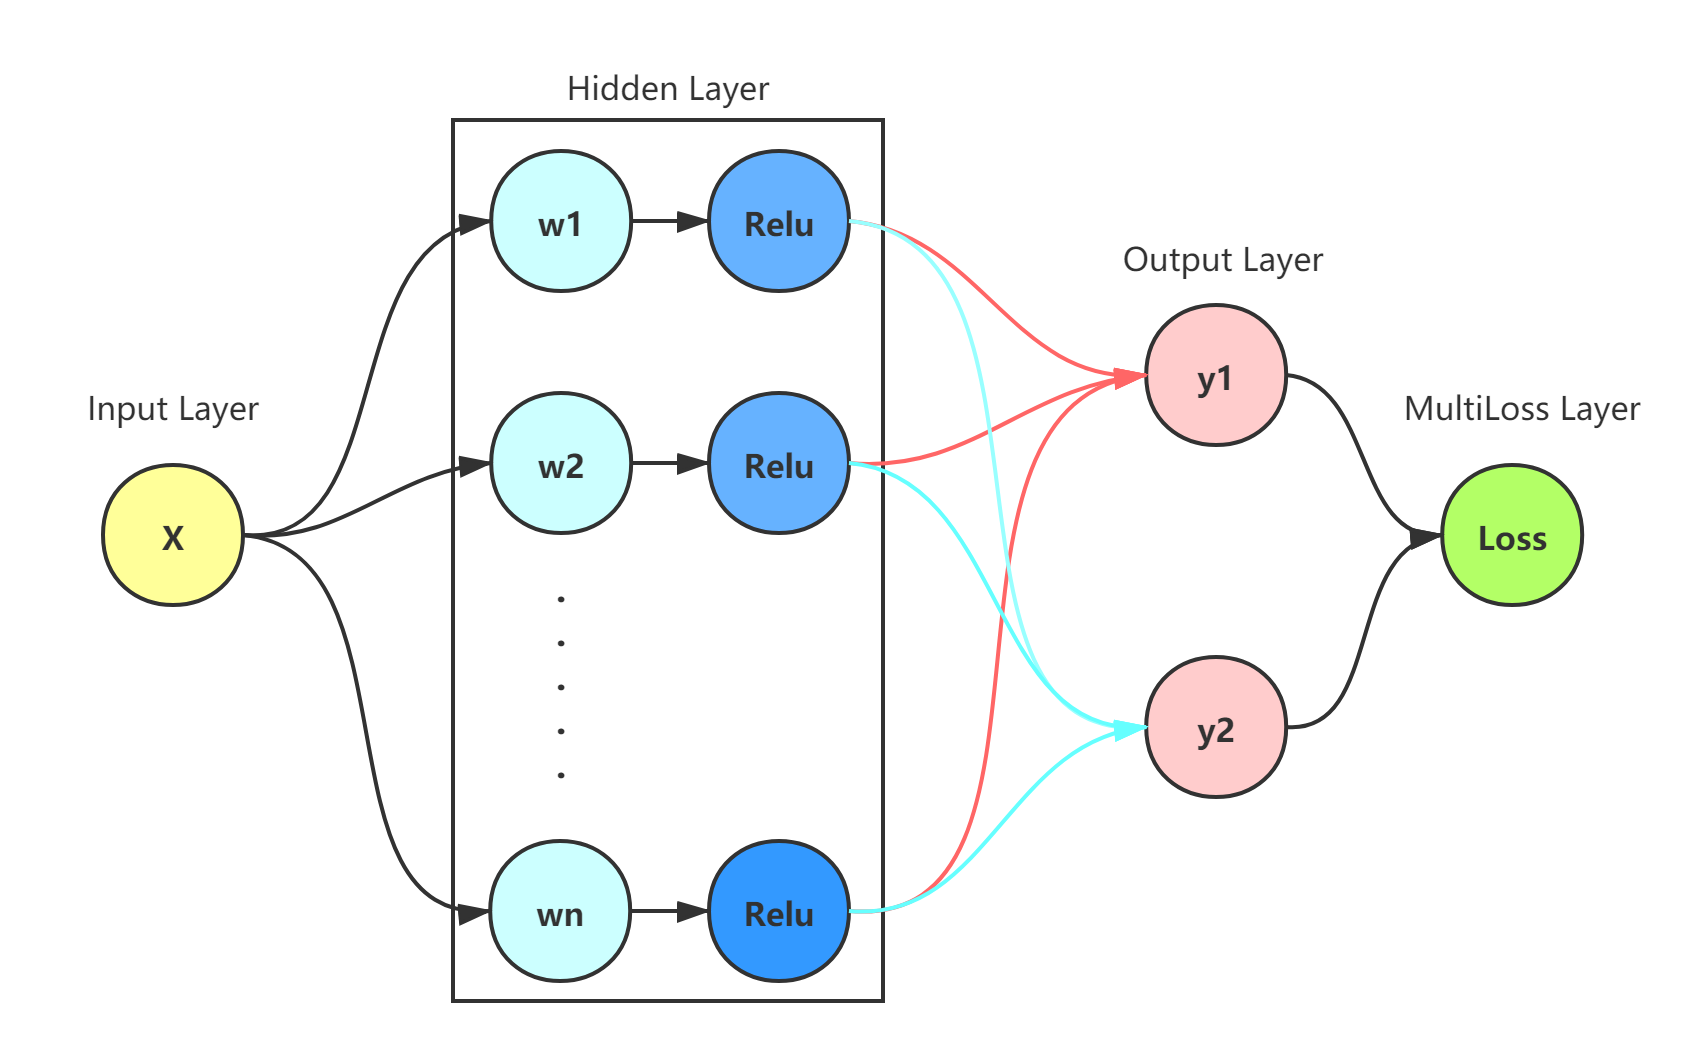
\includegraphics[width=5in]{figure/example/MultiLoss.png}\\
  \caption{多任务损失模型图}
  \label{fig:1-4}
\end{figure}

\subsection{小总结}

作者利用参考代码中简单的小例子,提出了一种多任务联合损失函数优化的方法(上面大部分小节都在讲这个损失函数的推导过程),并尝试将其应用在语义分割,实例分割,深度回归三个子任务所构成的总任务中,发现基于三个子任务的同方差不确定性损失加权效果最好。

一般来说,对于单任务输出的损失函数值是一个标量,而多任务的损失函数输出值是一个向量。如果损失函数值是一个向量的话,则需要通过线性求和来计算总的损失,即$L_{total}    = \sum_i w_i L_i$。在本文中,作者在基于回归任务的输出服从高斯分布,分类任务的输出服从玻尔兹曼分布的假设下,通过高斯似然和Softmax函数,定义了一个多任务联合损失函数(对数似然函数),通过最小化损失函数(最大似然估计)来确定这两个任务的参数,而非简单的线性加权求解参数。

整个任务的总体损失受不同重要因子的子任务共同影响。这个重要因子由输出数据的方差来决定,方差越大,信息不确定性越大,loss被赋予的权重也越大,进而应优先学习不确定性更大的子任务,使整个任务在全局输出上达到最优。

\subsection{补充知识}

\subsubsection{同方差不确定性}

在介绍相关知识前,先简单了解一下什么是"不确定性”。在很多情况下,深度学习领域都有极佳的表现,这种表现依赖于大量的数据,强大的算力,深厚的网络结构,会对某一个问题给出一个特定的答案,这个答案是给定模型在众多候选中找到概率最大的(比如分类问题最后用softmax)得到的,但是在极端情况下,答案的唯一输出会存在些问题。

如果训练的类别只包含A类和B类,但在测试阶段输入C 类的图片,那么分类器大概率会将自己所学到的类别作为输出结果,而这种错误,在容错率极低的行业,如航天,军事等领域,是绝不能容忍的。试想一下,如果面对这种极端情况,在输出结果的同时给出一个极低的相对于结果的置信度,这个低置信度会带来预警,让人为进行干预,效果会更好。这种置信度的输出,就要靠贝叶斯建模了。\\

在贝叶斯建模中,需要解决两种不同类型的不确定性。
\begin{enumerate}
    \item 认知不确定性:表示的是模型本身的不确定性,这是因为缺乏训练数据,模型认知不足,可以通过扩充训练集进行解决;
    \item 偶然不确定性:偶然不确定性表示数据不能解释的信息。举一个例子,在数据标注时如果出现比较大的标注误差,这个误差不是模型带入的,而是数据本身就存在的,数据集里的bias越大,偶然不确定性就越大。这也是贝叶斯派引入先验概率来修正原有数据在统计中产生误差的原因。
\end{enumerate}

偶然不确定性又分成两类:
\begin{enumerate}
    \item 数据依赖型或异方差不确定性(Data-dependent or Heteroscedastic uncertainty):这种不确定性取决于输入的数据,并且预测结果作为模型的输出。
    \item 任务依赖型或同方差不确定性(Task-dependent or Homoscedastic uncertainty):不取决于输入数据,而是取决于不同的任务。对于所有的输入数据,它们具有相同的常量,而对于不同的任务,它们有不同的变量。基于这个特性,我们称之为任务依赖型不确定性。
\end{enumerate}

因为在多任务学习中,任务的不确定性表明了任务间的相对置信度,反映了回归和分类问题中固有的不确定性。因此本文提出把同方差不确定性作为噪声来对多任务学习中的权重进行优化。\\

为了更好地理解后面提到的参考代码,这里先理解一下同方差的2个基本假设:
\begin{enumerate}
    \item 假设一被称为(White Noise Condition)白噪音假设,干扰项即误差部分相互没有关联。假设回归式$y=\alpha + \beta x + u$, 其误差项中,$u1,u2$各误差之间没有任何联系,即:协方差矩阵$COV(u1 * u2)= 0$。
    \item 假设二为干扰项具备同方差性或者等分散, 即误差项与独立变量(independent variable)之间相互独立, 并且误差项的分散(方差)必须等同,即$Var(u|x)=\sigma^2$;解释变量之间不存在多重共线性;解释变量是确定变量。
\end{enumerate}

\subsubsection{频率派和贝叶斯派}

在概率估计或者机器学习里的参数估计上,有两个方法,MLE(最大似然估计) 和MAP(最大后验估计),其实代表了概率论里的两个派别,频率派和贝叶斯派\footnote{频率派vs贝叶斯派 \quad \url{https://blog.csdn.net/weixin_43593330/article/details/105797717}}。 在了解这两个派别所研究内容有啥区别之前,我们有必要先理清一些基础概念:什么是似然函数,什么是概率函数,什么是MLE,MAP。\\

1、似然函数 和 MLE(最大似然估计)

在统计学中,假设我们对含未知参数的模型给定一个参数值,似然函数可以用来衡量这个模型对于数据样本的拟合程度。似然函数由样本的联合概率分布构成,并作为关于参数的函数。通过似然函数最大化来求解这些参数,即最大似然估计。为了计算方便,通常使用对数似然函数。在概率论的两个派别中,似然函数都起着基础性的作用。\\

在MLE中,首先要定义似然函数$$
\begin{align}
& L(\theta|x) = f_D(x_1,x_2,...,x_n|\theta) \nonumber \\
& = \prod_{i = 1}^n p(x_i;\theta)
\end{align}

在$\theta$的所有取值上,使这个函数最大化,这个使可能性最大的值即为MLE(一般求解步骤见Wiki)。

这里举个例子:假设有一个造币厂生产某种硬币,现在我们拿到了一枚硬币,想试试这硬币是不是均匀的,我们可以通过抛硬币的方式,统计硬币正反面出现的概率(记为$\theta$),如果正反面出现的概率相同,则该硬币是均匀的,反之亦然\footnote{贝叶斯公式理解与应用 \quad \url{https://blog.csdn.net/qq_33934427/article/details/105002894}}。

于是我们拿这枚硬币抛了10次,得到的数据($x_0$)是:"反正正正正反正正正反",其中正面概率$\theta$是我们想求的模型参数,我们可以得到似然函数
\begin{align}
& f(x_0,\theta)=(1-\theta) \times \theta \times \theta \times \theta \times \theta \times (1-\theta) \times \theta \times \theta \times \theta \times (1-\theta)=\theta^7(1-\theta)^3 = f(\theta)
\end{align}

实验得到的似然函数值为0.7,这能说明该厂生产的硬币是不均匀吗?显然是不行的,实验的次数太少了,如果实验次数达到上千次,正负面统计的频数或许各占一半。\\

2、MAP(最大后验估计)

最大似然估计通过求解参数$\theta$, 使似然函数$P(x0|\theta)$最大。而最大后验概率估计则是在求解$\theta$过程中,使$P(x0|\theta)P(\theta)$最大。要想使后验概率尽可能大,关于$\theta$的似然函数要大,$\theta$自己出现的先验概率也要大。这有点像正则化里加惩罚项的思想,不过正则化里是利用加法,而MAP里是利用乘法。MAP公式如下

\begin{align}
& P(\theta|x0)=\frac{P(x0|\theta)P(\theta)}{P(x0)}
\end{align}

由于MAP在计算过程中,$x0$是确定的。如果还是拿上面MLE的例子,$x0$ 表示硬币投出正反面数:“反正正正正反正正正反”,假设“投10次硬币”是一次实验,实验做了1000 次,“反正正正正反正正正反”出现了n次,则$P(x0)=n/1000$。因此$P(x0)$是一个已知值,所以在计算MAP时可以去掉分母$P(x0)$

MAP在最大化$P(\theta|x0)$ 的意义也很明确,$x0$已经确定了,求$\theta$ 使$P(\theta|x0)$ 最大。\\

3、概率函数和似然函数

对于如下函数,假设输入有两个:$x$表示某一个具体的数据; $\theta$ 表示模型的参数。
\begin{align}
& P(x|\theta)
\end{align}

若$\theta$是已知确定的,$x$是变量,这个函数叫做概率函数,它描述在给定模型参数$\theta$,对于不同的样本点$x$其出现概率是多少(softmax)。最大后验概率估计目的是求$x$,即
\begin{align}
& p(X|\theta) = \max\{p(x_1 | \theta),p( x_2 | \theta), ... , p( x_3 | \theta)\}
\end{align}

如果$x$是已知确定的,$\theta$是变量,这个函数叫做似然函数,它描述对于不同的模型参数,出现$x$这个样本点的概率是多少。最大似然估计目的是求参数$\theta$,即
\begin{align}
& p(X|\theta) = \max\{p(X | \theta_1),p( X | \theta_2), ... , p( X | \theta_n)\}
\end{align}

\quad

4、统计和概率的区别:

概率(probabilty)和统计(statistics)看似两个相近的概念,其实研究的问题刚好相反。
\begin{itemize}
    \item 概率研究的问题是,已知一个模型和参数,怎么去预测这个模型产生的结果的特性(例如均值,方差,协方差等等)
    \item 统计研究的问题是,有一堆数据,要利用这堆数据去预测模型和参数。
\end{itemize}

一句话总结:概率是已知模型和参数,推数据。统计是已知数据,推模型和参数。\\

5、小总结

往大的说,这两个派别代表了不同的世界观。频率派认为参数($\theta$) 是客观存在不会改变的,虽然未知,但却是固定值。贝叶斯派则认为参数是随机值,因为不可能做完整的实验去确定,因此参数也可以有分布。

往小处说,频率派最常关心的是似然函数,他们认为直接用样本去计算出的概率就是真实的,而贝叶斯派最常关心的是后验分布,他们认为样本只是用来修正经验观点。

贝叶斯派因为所有的参数都是随机变量,都有分布,因此可以使用一些基于采样的方法 (如MCMC)使得我们更容易构建复杂模型。频率派的优点则是没有假设一个先验分布,因此更加客观,也更加无偏,在一些保守的领域(比如制药业、法律)比贝叶斯方法更受到信任。

本质上MLE是根据样本数据直接计算概率参数,而MAP是预设一个参数的概率分布,然后通过样本数据去进行修正。如果样本量不够大的时候,MAP 可能更符合人们的日常经验,比如一个硬币抛五次,都是正面朝上,那么MLE算出来就是这个硬币正面朝上概率为100$\%$,而用先验概率50$\%$加上MAP去算,可能只是51$\%$,更符合人们的日常经验。

如果样本量足够大,这两个方法还是殊途同归的,都是进行参数估计。如果样本量适中,那么MAP使用比较合理的先验概率是很重要的。 \\

6、谈谈我的理解

最大似然估计和最大后验概率,它们两者目的一致,都是为了进行参数估计。频率派认为数据样本是客观可靠的,相信从中统计样本可以进行参数估计,因此最大似然估计则是在给定样本中计算最大的联合概率,求解这个参数,该参数模型对数据样本拟合最好。

而贝叶斯派认为数据样本不可靠,单纯通过对数据样本的统计可能会存在问题,因此最大后验概率需要先给定某个参数的先验概率(这个先验概率可以通过专家讨论得到)作为”正则化项”,来修正通过数据样本计算似然函数时存在的不准确的问题

核心思想搞懂了,再来看看MLE,MAP在计算中,谁是已知的,谁是未知的,这样才不容易搞混:MLE中参数未知,x已知(因为对数据样本统计求解参数),MAP中参数已知(有先验概率),x未知(x不可靠,需要利用先验概率来修正似然函数),最终目的都是为了求解最优参数(参数是个广泛的概念,比如硬币的正反面,单词的含义等)。


